\chapter{Implementation and reproducibility}
\label{app:rep}
\section{Data lineage}
The experiment snapshot for this thesis is \texttt{6031e3f}. The frozen run used commit \texttt{e6a375d}, with its machine lock published in \texttt{3afce6a} before opening the test data. The private project includes the complete protocol and small results alongside the code \cite{project}. It excludes the original tables, learned weights and credentials. Exact regeneration requires access to the original tables and weights. The LaTeX project includes the figure assets and tables required to compile the document without that access.

The network file is identified by SHA-256 prefix \texttt{a06b5c0765fb2d49}. The locked machine manifest has prefix \texttt{2ef4bddc8b727bc5}. These prefixes identify the full hashes in the experiment records. Changing a lane connection or polyline can alter a route while leaving the filename unchanged. The code checks paths, counts and weights so that two variants cannot silently consume different inputs.

\tab{Execution stages. An empirical seed selects a resampling realization, whereas a training seed identifies a separately fitted network.}{work}{\begin{tabularx}{\linewidth}{lX}\toprule Stage & Unit of work\\\midrule
E1 & 12 auxiliary CNN fits. Two grids, two initialization choices and three seeds. Full-vehicle classification.\\
E2 & Nine horizon-matched CNN fits plus transfer evaluation. Three horizons, three seeds and one common validation cohort.\\
E3 & Three motion diffusion models, 20,000 updates each. Each produces 511 incremental distances.\\
E4/E4r & Three raw-coordinate TCN fits, shared masks, fixed versus independent candidate paths and shuffled-target controls.\\
E3b & Three empirical motion resamplings on the same paths.\\
E5 & Six groups, two downstream architectures and three seeds. Thirty-six fixed-budget learner fits.\\
E7 & Lock manifest, checks, one held-out evaluation, conditional bootstrap, copy control and exports.\\\bottomrule\end{tabularx}}
The historical short-horizon coordinate and displacement-image studies explain why the representation was changed. Their validation numbers refer to different data and are kept separate from the formal long-window results.

\section{Run parameters}
\tab{Parameters of the main comparison. The actual length of a path can be smaller than its budget.}{params}{\begin{tabularx}{\linewidth}{lX}\toprule Item & Locked value\\\midrule
Horizon & 512 samples at 0.25 seconds, 511 increments\\
Path & Up to 4,096 m and 1,025 interpolation points\\
Successor prior & Class-conditioned counts, 0.1 smoothing per permitted successor\\
Denoiser & Width 128 with ten dilated residual blocks, class, start, time and route conditions\\
Noise & 1,000 linear schedule steps, 100-step DDIM at generation\\
Generator & Final averaged weights, seeds 42/43/44\\
Candidate budget & Eight per request per seed, shared paths and ordered noise\\
Path and noise seeds & 20261109 and 20261110\\
Selection seed & 20261111 for priority and target shuffle\\
Paired resampling & 2,000 draws, seeds 20261112 (motion) and 20261113 (downstream)\\
Augmentation & One generator, training paths only, 425 selected per variant\\
Downstream & Seeds 100/101/102, fixed 1,150 updates at batch size 64\\
\bottomrule\end{tabularx}}
When computing a paired interval, the same resampled participant multiplicities apply to all seeds. Treating all 1,272 generated samples as independent bootstrap units would represent the original 53 references many times without corresponding new information about the population.

\section{Reference and request interfaces}
Preparation reads the assigned test participants, identifies their continuous segments, attempts image encoding and road reconstruction and writes references and requests separately. The request interface permits the start and class. Indices relate a request to its reference during evaluation. Planning consumes requests and training-side transition counts. Sampling consumes planned routes, starts, labels and frozen weights.

This separation can be tested without a real vehicle. One interface test presents a request with an unexpected future-path field and expects rejection. A budget test supplies a condition with one planning failure among eight slots and expects an unserved request. A file-integrity test changes a locked file and expects verification to fail before scoring. The full lock manifest and completion markers identify which run produced the results.

\section{Coordinate export specification}
Each output row has the fields \texttt{time,id,x,y,type}. The first sample of each track has relative time zero and the last has time 127.75 seconds. Coordinates are local MoST metres. The machine-readable bicycle class retains its historical spelling \texttt{bycicle}. Synthetic identities distinguish samples even when several samples share a start.

The training archive contains the exact extras used in E5. Each of the random, image-selected and TCN-selected variants contains 425 trajectories or 217,600 rows. Their coordinates and labels match the synthetic tail of the corresponding training arrays, and parent IDs belong to the training split. Alternatives originate in one common candidate pool, so combining all versions would count some samples several times.

The final-condition archive contains all 1,272 diffusion candidates and four selected variants of 159 trajectories each. Each selected file takes one sample per condition per generator seed. Counts, finite coordinates and timestamps were verified by reading the exports back. Archive hashes identify the exact files. A new model trained with these final-condition traces would require a new independent evaluation population.

\chapter{Class evidence and fixed trajectory examples}
\label{app:cases}
The five panels below use the first served condition per class at generator seed 42, the rule used in Figure~\ref{fig:map}. Their labels refer to the same candidate indices as the recorded map-example manifest. The panels show speed and cumulative planar travel for all eight synthetic candidates. Highlighting the image-selected trace connects the map view to differences in timing. Each accompanying class table uses all available test conditions for that class and all three frozen seeds. Thus the table describes the full class-specific distributions, while the curves describe one particular request.

\begingroup
\renewcommand{\tab}[3]{\begin{table}[H]\centering\caption{#1}\label{tab:#2}\small #3\end{table}}
\clearpage\section{Bus}
Buses supply seven reference conditions. Empirical transfer reproduces the observed stop fraction more closely in this class, yet its travel-distance discrepancy is larger. A closer match in the total time spent nearly stationary does not specify where those stationary intervals occur or how far the vehicle travels between them.

The fixed request contains eight candidates. The random, image and coordinate rules returned candidate indices 4, 4 and 7, respectively. The observed class stop fraction across the 7 references is 29.5\%.

\begin{center}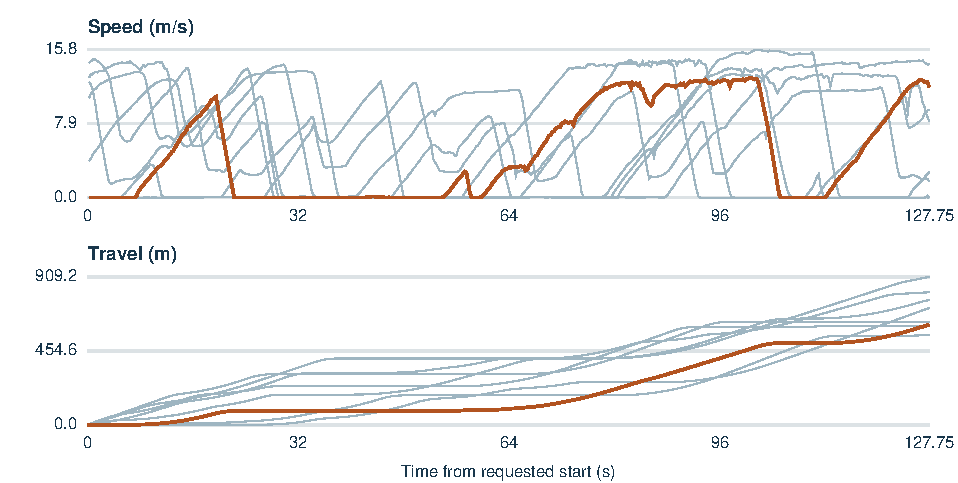
\includegraphics[width=.98\linewidth]{figures/case-bus.pdf}\end{center}
\noindent The highlighted line is the GAF-selected trace. The seven other trajectories are shown in blue-gray. Axes are scaled separately for each class.
\tab{All-candidate bus results. Units are m/s, m/s$^2$, m and percent, respectively.}{case1}{\begin{tabular}{lrrrr}\toprule
Motion & Speed $\W$ & Accel. $\W$ & Travel $\W$ & Stop \%\\\midrule
Diffusion & 0.736 & 0.078 & 95.242 & 22.3\\
Empirical & 0.985 & 0.108 & 180.760 & 31.4\\\bottomrule\end{tabular}}
\FloatBarrier

\clearpage\section{Motorcycle}
The four motorcycle references spend roughly a quarter of sampled intervals below the stop threshold. Both generators spend only about seven percent. Transporting observed profiles from the training library therefore leaves a substantial mismatch even before a learned motion distribution is used. Whether the gap reflects different route mixes or insufficient training coverage requires independent conditions.

The fixed request contains eight candidates. The random, image and coordinate rules returned candidate indices 119, 116 and 115, respectively. The observed class stop fraction across the 4 references is 24.6\%.

\begin{center}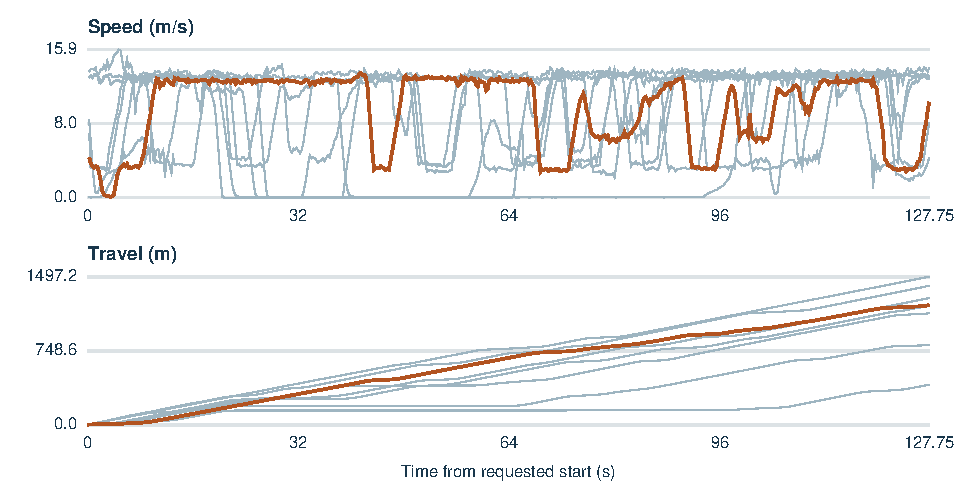
\includegraphics[width=.98\linewidth]{figures/case-motorcycle.pdf}\end{center}
\noindent The highlighted line is the GAF-selected trace. The seven other trajectories are shown in blue-gray. Axes are scaled separately for each class.
\tab{All-candidate motorcycle results. Units are m/s, m/s$^2$, m and percent, respectively.}{case2}{\begin{tabular}{lrrrr}\toprule
Motion & Speed $\W$ & Accel. $\W$ & Travel $\W$ & Stop \%\\\midrule
Diffusion & 2.068 & 0.199 & 347.655 & 7.0\\
Empirical & 2.758 & 0.265 & 367.777 & 7.4\\\bottomrule\end{tabular}}
\FloatBarrier

\clearpage\section{Private car}
Private cars account for 33 of the 53 requests. Their stop fraction is closely matched by diffusion, and their travel discrepancy is smaller than with empirical transfer. The empirical baseline, however, gives a much smaller acceleration discrepancy for this class. These results distinguish agreement on total distance from agreement on changes in speed.

The fixed request contains eight candidates. The random, image and coordinate rules returned candidate indices 133, 133 and 135, respectively. The observed class stop fraction across the 33 references is 4.8\%.

\begin{center}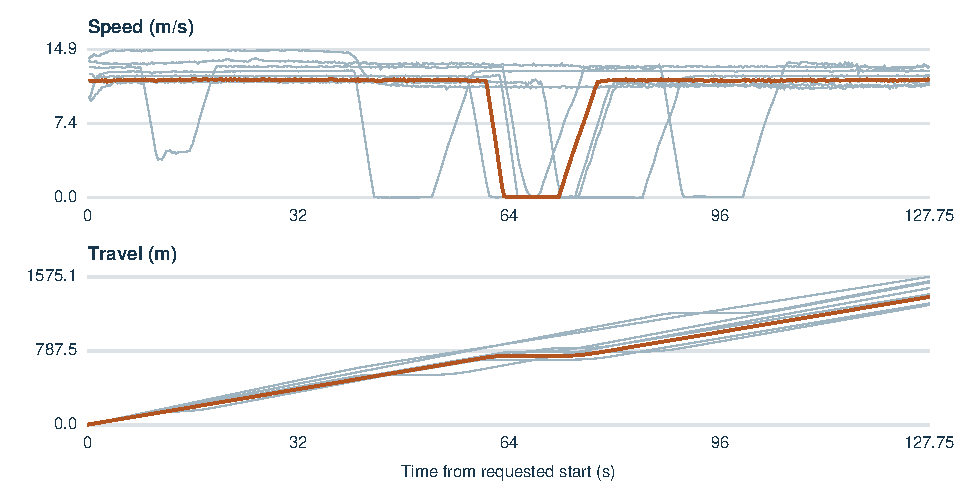
\includegraphics[width=.98\linewidth]{figures/case-private_car.pdf}\end{center}
\noindent The highlighted line is the GAF-selected trace. The seven other trajectories are shown in blue-gray. Axes are scaled separately for each class.
\tab{All-candidate private car results. Units are m/s, m/s$^2$, m and percent, respectively.}{case3}{\begin{tabular}{lrrrr}\toprule
Motion & Speed $\W$ & Accel. $\W$ & Travel $\W$ & Stop \%\\\midrule
Diffusion & 0.356 & 0.187 & 51.620 & 4.8\\
Empirical & 0.985 & 0.058 & 124.766 & 3.8\\\bottomrule\end{tabular}}
\FloatBarrier

\clearpage\section{Bicycle}
The seven observed bicycle windows spend little sampled time below the stop threshold. The two generators produce similar stop fractions of about three percent. Both acceleration discrepancies are comparatively large. Since acceleration here differentiates planar speed, quarter-second variations in the decoded geometry and timing can affect this metric even on a connected route.

The fixed request contains eight candidates. The random, image and coordinate rules returned candidate indices 62, 59 and 61, respectively. The observed class stop fraction across the 7 references is 0.1\%.

\begin{center}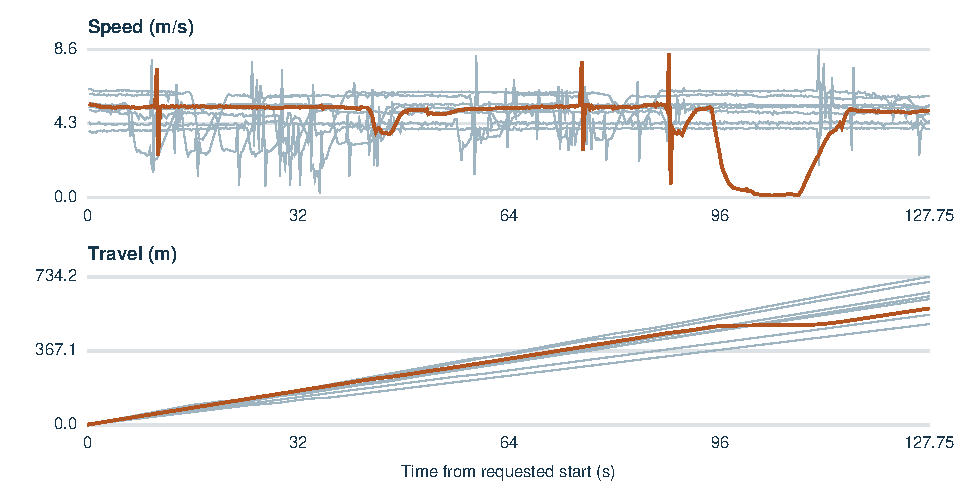
\includegraphics[width=.98\linewidth]{figures/case-bycicle.pdf}\end{center}
\noindent The highlighted line is the GAF-selected trace. The seven other trajectories are shown in blue-gray. Axes are scaled separately for each class.
\tab{All-candidate bicycle results. Units are m/s, m/s$^2$, m and percent, respectively.}{case4}{\begin{tabular}{lrrrr}\toprule
Motion & Speed $\W$ & Accel. $\W$ & Travel $\W$ & Stop \%\\\midrule
Diffusion & 0.378 & 0.651 & 55.534 & 3.0\\
Empirical & 0.505 & 0.607 & 74.275 & 3.0\\\bottomrule\end{tabular}}
\FloatBarrier

\clearpage\section{Taxi or Uber}
Only two taxi requests supply the reference distribution. In this class empirical transfer has smaller speed and travel discrepancies than diffusion, while both generators spend considerably less time nearly stationary than the two observed vehicles. The direction of the class-specific result is informative, but two vehicles provide very little information about the broader taxi population.

The fixed request contains eight candidates. The random, image and coordinate rules returned candidate indices 247, 241 and 247, respectively. The observed class stop fraction across the 2 references is 19.2\%.

\begin{center}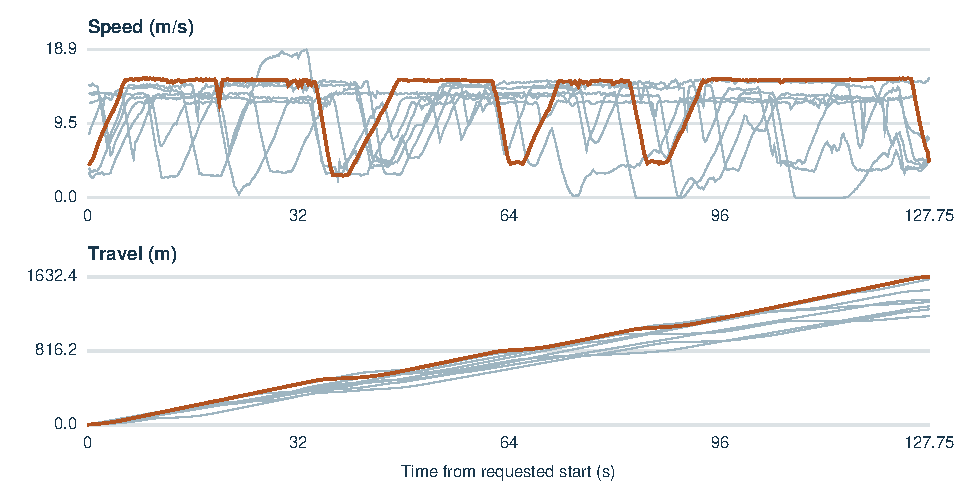
\includegraphics[width=.98\linewidth]{figures/case-taxi_or_uber.pdf}\end{center}
\noindent The highlighted line is the GAF-selected trace. The seven other trajectories are shown in blue-gray. Axes are scaled separately for each class.
\tab{All-candidate taxi or uber results. Units are m/s, m/s$^2$, m and percent, respectively.}{case5}{\begin{tabular}{lrrrr}\toprule
Motion & Speed $\W$ & Accel. $\W$ & Travel $\W$ & Stop \%\\\midrule
Diffusion & 2.681 & 0.231 & 337.019 & 2.2\\
Empirical & 2.000 & 0.155 & 258.019 & 5.3\\\bottomrule\end{tabular}}
\FloatBarrier

\endgroup

\chapter{Detailed classification and selection results}
\label{app:classification}
\section{Auditor confusion and imbalance}
The confusion summaries retain errors hidden by aggregate accuracy. Each matrix averages the row proportions of three separately trained networks on the same 182 vehicles. A cell is the share of participants of the true class predicted as the column class. Row counts are 12, 13, 31, 103, 15 and 8. An error on one taxi changes taxi recall by 12.5 points for one model.

\fig{confusion.pdf}{1}{Final auxiliary classification on observed windows. Rows are true classes and columns are predictions. Each cell averages percentages across the three frozen seeds.}{confusion}
\tab{Observed-window recognition by class. Recall and F1 are given as percentages}{auxclasses}{\begin{tabular}{lrrrrr}\toprule
Class & IDs & GAF recall & GAF F1 & TCN recall & TCN F1\\\midrule
Pedestrian & 12 & 80.6 & 85.3 & 100.0 & 98.7\\
Bus & 13 & 76.9 & 77.1 & 82.1 & 69.1\\
Motorcycle & 31 & 40.9 & 36.2 & 59.1 & 58.1\\
Private car & 103 & 75.4 & 78.0 & 82.2 & 83.8\\
Bicycle & 15 & 46.7 & 43.6 & 100.0 & 100.0\\
Taxi or Uber & 8 & 0.0 & 0.0 & 29.2 & 27.8\\\bottomrule\end{tabular}}

These matrices use observed-window recognition. The audit percentages on generated traces use requested classes on the five-class subset and two audit seeds per family. Accuracy across observed windows, six-class macro-F1 and class-macro agreement on generated candidates measure different outcomes.

\section{The complete selection comparison}
\tab{Locked five-class macro results by motion model and selection rule. Units are m/s, m/s$^2$, m and percent.}{fullselection}{\begin{tabular}{llrrrrr}\toprule
Motion & Rule & Speed & Accel. & Travel & GAF & TCN\\\midrule
Diffusion & All candidates & 1.24 & 0.27 & 177.41 & 47.48 & 77.68\\
 & Random & 1.40 & 0.28 & 206.00 & 51.85 & 89.86\\
 & GAF & 1.41 & 0.29 & 191.52 & 70.45 & 78.10\\
 & TCN & 1.44 & 0.29 & 209.30 & 47.32 & 93.18\\
 & Shuffled GAF & 1.50 & 0.28 & 195.80 & 39.55 & 76.95\\
Empirical & All candidates & 1.45 & 0.24 & 201.12 & 40.47 & 71.07\\
 & Random & 1.69 & 0.26 & 233.89 & 45.61 & 78.17\\
 & GAF & 1.89 & 0.28 & 252.55 & 63.11 & 68.41\\
 & TCN & 2.28 & 0.31 & 282.14 & 42.72 & 91.36\\
 & Shuffled GAF & 1.49 & 0.27 & 195.02 & 35.41 & 63.04\\\bottomrule\end{tabular}}

The complete-candidate row describes the distribution available to each selector. The single-selection rows serve one trace per request and therefore also use fewer samples. A difference between the full-pool and random rows alone is not an effect of feedback. The direct comparator for GAF ranking is random ranking within the same saved pool.

\section{Paired downstream contrasts}
\tab{GAF-selected augmentation minus each comparator in macro-F1 percentage points, with 95\% paired intervals}{contrasts}{\begin{tabular}{lrr}\toprule
Comparator & TCN & GRU\\\midrule
Observed only & -5.23 [-9.01, -1.65] & -1.70 [-6.42, +3.13]\\
Repeat & -1.09 [-4.02, +1.93] & +2.98 [+0.28, +5.95]\\
Time warp & -1.63 [-4.42, +1.33] & -0.46 [-2.77, +2.16]\\
Random synthetic & +1.40 [-1.54, +5.16] & +1.86 [-1.70, +5.47]\\
GAF synthetic & +0.00 [+0.00, +0.00] & +0.00 [+0.00, +0.00]\\
TCN synthetic & -0.39 [-4.41, +4.26] & +1.48 [-1.72, +4.82]\\\bottomrule\end{tabular}}

The comparison with repeated data concerns a change in motion while maintaining parent counts and class inventory. The comparison with randomly selected synthetic data isolates the value of choosing an image-preferred candidate. The comparison with observed-only training measures the practical effect of the delivered augmentation package as a whole.

\section{Per-class downstream outcomes}
\tab{Downstream per-class recall on the observed test set, in percent. Entries average the three learner initializations.}{recall}{\begin{tabular}{llrrrrrr}\toprule
Model & Group & Ped. & Bus & Moto. & Car & Bike & Taxi\\\midrule
TCN & Observed only & 100.0 & 84.6 & 51.6 & 82.5 & 100.0 & 62.5\\
 & Repeat & 88.9 & 89.7 & 48.4 & 82.8 & 100.0 & 45.8\\
 & Time warp & 91.7 & 89.7 & 48.4 & 83.5 & 100.0 & 45.8\\
 & Random synthetic & 86.1 & 92.3 & 48.4 & 82.2 & 100.0 & 33.3\\
 & GAF synthetic & 100.0 & 92.3 & 43.0 & 80.3 & 100.0 & 45.8\\
 & TCN synthetic & 83.3 & 89.7 & 51.6 & 82.8 & 100.0 & 37.5\\
GRU & Observed only & 100.0 & 41.0 & 37.6 & 81.9 & 95.6 & 66.7\\
 & Repeat & 88.9 & 46.2 & 30.1 & 81.2 & 93.3 & 58.3\\
 & Time warp & 88.9 & 53.8 & 33.3 & 80.9 & 97.8 & 62.5\\
 & Random synthetic & 86.1 & 51.3 & 31.2 & 81.9 & 95.6 & 58.3\\
 & GAF synthetic & 100.0 & 59.0 & 30.1 & 78.6 & 95.6 & 62.5\\
 & TCN synthetic & 86.1 & 53.8 & 35.5 & 79.9 & 97.8 & 54.2\\\bottomrule\end{tabular}}

The downstream task keeps pedestrians in evaluation although augmentation adds no pedestrian traces. Their recall can therefore change: adding examples of other classes changes the learned decision boundary. Improved recall in a class can also come at the expense of precision if the learner predicts the class more often. Consequently the primary six-class evaluation uses macro-F1, with per-class recall as a diagnostic.

\section{Sensitivity of the evidence}
The network could be retrained, the planner and motion sampler could draw new candidate pools, and a different set of participants could be observed. Only the last component enters the paired intervals, conditional on the existing models and routes. Resampling test participants cannot estimate sensitivity to another city or simulator version.

The whole-profile copying control has a specific interpretation. Time alignment is fixed, all 511 increments enter equally and error is measured in metres per increment. A copied short maneuver within an otherwise novel trajectory could escape detection. Two naturally similar motion sequences could also agree under a looser threshold. The empirical positive control and held-out reference comparison make the operational threshold interpretable in this study.
